\documentclass{article}
%% GRAPH OF TRAFFIC CIRCLE
\usepackage[usenames,dvipsnames]{xcolor}
\usepackage{tikz}
\usetikzlibrary{arrows}
\begin{document}
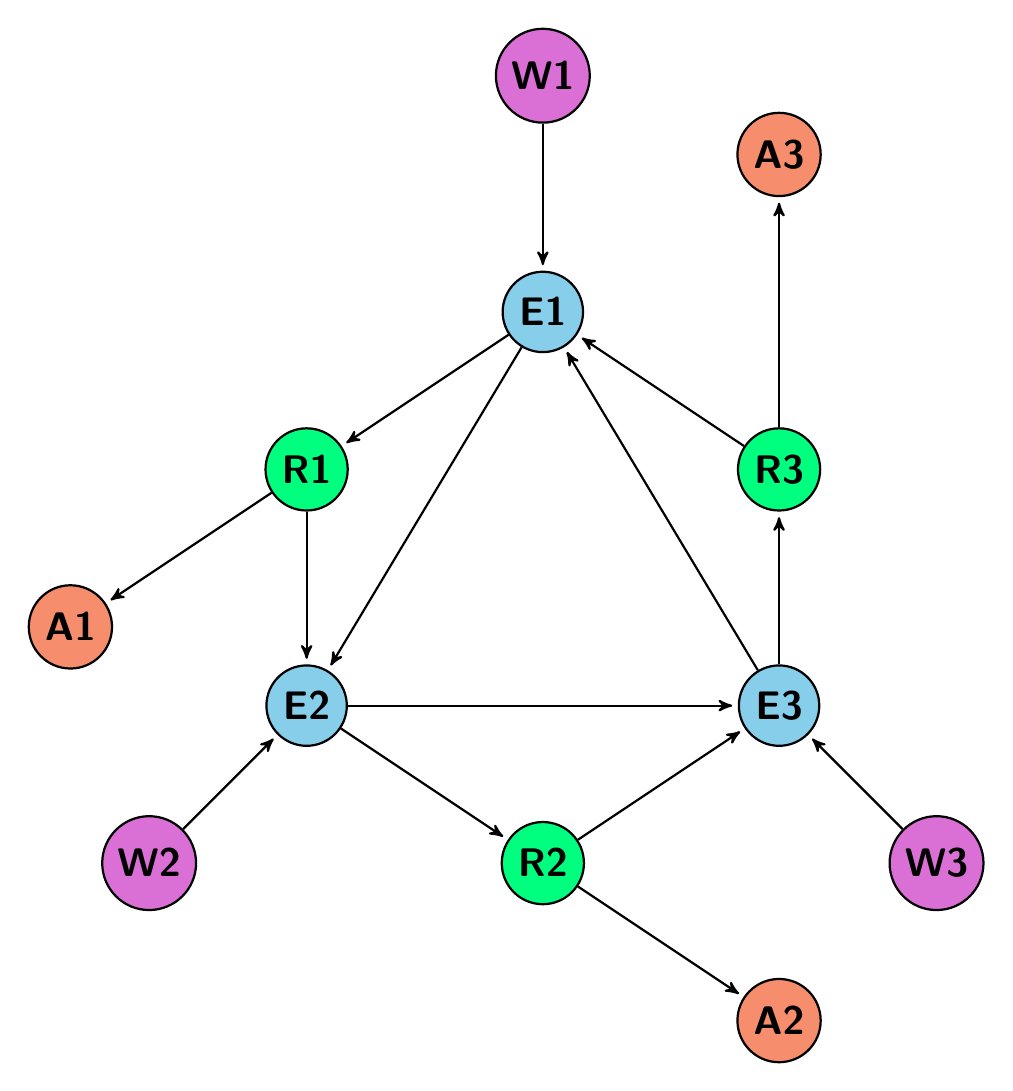
\begin{tikzpicture}[->, >=stealth', shorten >=2pt,auto,node distance=4cm, thick, exit/.style={circle, draw, fill = Melon, font = \sffamily\Large\bfseries}, enter/.style={circle, draw, fill = SkyBlue, font = \sffamily\Large\bfseries}, right turn/.style={circle, draw, fill = SpringGreen, font = \sffamily\Large\bfseries}, wait line/.style={circle, draw, fill = Orchid, font = \sffamily\Large\bfseries}]

\node[right turn] (R1) at (2,8) {R1};
\node[right turn] (R2) at (5,3) {R2};
\node[right turn] (R3) at (8,8) {R3};

\node[enter] (E1) at (5,10){E1};
\node[enter] (E2) at (2,5){E2};
\node[enter] (E3) at (8,5) {E3};

\node[exit] (A1) at (-1,6){A1};
\node[exit] (A2) at (8,1){A2};
\node[exit] (A3) at (8,12){A3};

\node[wait line](W1) at (5,13){W1};
\node[wait line](W2) at (0,3){W2};
\node[wait line](W3) at (10,3){W3};

\foreach \from/\to in {E1/R1,R1/A1,R1/E2,E1/E2,E2/R2,E2/E3,R2/A2, E3/E1,E3/R3,R3/E1,R3/A3,R2/E3,W1/E1, W2/E2, W3/E3} 
    \draw (\from) -- (\to);
\end{tikzpicture}
\end{document} 